Voici un tableau de variations.

\begin{tikzpicture}
\tkzTabInit[lgt=1,espcl=2]{ $x$ / 1,$f $ / 2}
{ $-4$ , $-2$ ,1,3}
\tkzTabVar{-/$-3$,+/$-1$,-/$-2$,+/$1$ }
\end{tikzpicture}

Pour chacune des affirmations, dire si elle est VRAIE ou FAUSSE. Justifier.

\begin{enumerate}
\item Pour tout réel $x$, tel que $-4 \leq x \leq 3$, on a $f(x) \leq 3$
\item Il existe un réel $x$, $x \in [-4;1]$ tel que $f(x) \geq 0$
\item Pour tout réel $x$, tel que $-4 \leq x \leq 3$, on a $f(x) \geq -4$
\item Il existe un réel $x$, $x \in [-4;1]$ tel que $f(x) \leq -4$
\item Pour tout réel $x$, tel que $-2 \leq x \leq 3$, on a $f(x) \leq 0$ 
\end{enumerate}
